\documentclass[a4paper,10pt]{report}
\usepackage[utf8]{inputenc}
\usepackage{amssymb}
\usepackage{amsthm}
\usepackage{amsmath}
\usepackage{graphicx}

\setlength{\parindent}{0pt}

\begin{document}
\title{Modern Physics - Waves, Optics}
\author{Zack Garza}
\maketitle
\tableofcontents

\chapter{Geometric Optics}
\section{Reflection}
\begin{enumerate}
 \item Specular Reflection

 Reflection from a smooth surface that reflects rays parallel to each other. Occurs as long as the surface variations are much smaller than $\lambda$.

 \item Diffuse Reflection

 Reflection from a rough surface that reflects rays in various directions.

\end{enumerate}

In general, the angle of reflection will equal to angle of incidence, or
\begin{align*}
 \theta_{1}' &= \theta_1 \\
 (\text{Reflection Angle} &= \text{Incident Angle})
\end{align*}


\section{Refraction}
\subsection{Flat Refracting Surfaces}

\begin{figure}[h!]
  \begin{centering}
  \begin{center}
  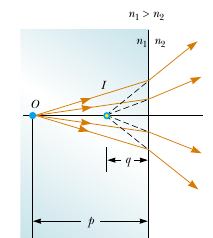
\includegraphics{./flat_refracting.png}
  \caption{Image formed by a flat refracting surface.}
  \label{fig:flat_refracting}
  \end{center}
  \par\end{centering}
  \end{figure}

See Figure~\ref{fig:flat_refracting}. The equation generally used is
\begin{align*}
  \frac{n_1}{p} = \frac{-n_2}{q}
\end{align*}
Where $-q$ denotes the distance from the surface to the image. The image formed is also always on the same side of the surface as the object itself.

\subsection{Equations}
\begin{enumerate}
  \item
    Index of Refraction:
    \begin{align*}
        n &= \frac{c}{v_{\text{Medium}}} \text{ or } vn=c
    \end{align*}
    Defined as the ratio between the speed of light in a vaccum and in a medium. $v$ is always less than $c$, so $n>1$ for all substances.
    This also implies $\lambda_n < \lambda$, or that the wavelength of light in a medium is always lower than its wavelength in a vacuum.

  \item
    Snell's Law of Refraction:
    \begin{align*}
    n_1\sin\theta_1 &= n_2\sin\theta_2 \\
    \lambda_1 n_1 &= \lambda_2 n_2
    \end{align*}
    As light travels from one medium to another, its frequency does not change, but its wavelength \underline{does}.

  \item
    Total internal reflection:
    \begin{align*}
     &\sin\theta_{\text{crit}} = \frac{n_2}{n_1} &(\text{for } n_1 > n_2)
    \end{align*}
    Occurs when light travels from a medium with a high $n$ to one with a lower $n$, so $n_2/n_1 \le 1$.
    Can be in degrees or radians, just use the conversion
    \begin{align*}
     \frac{\text{radians}}{2\pi} = \frac{\text{degrees}}{360^{\circ}}
    \end{align*}
\end{enumerate}

\chapter{Image Formation: Mirrors, Lenses}

\section{Flat Mirrors}
  \begin{figure}[htpb]
  \begin{centering}
  \begin{center}
  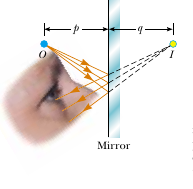
\includegraphics[]{./pqmirror.png}
  \label{fig:parallel_diagram}
  \caption{Conventions}
  \end{center}
  \par\end{centering}
  \end{figure}
  Conventions
  \begin{itemize}
   \item $O$: Object
   \item $I$: Image of object
   \item $p$: Actual distance of object
   \item $q$: Distance of Image
  \end{itemize}

\section{Conic Mirrors}
To determine image location, only three principle rays are essential:
\begin{enumerate}
 \item
    From the top of the object, parallel to the principal axis.

    (Reflected along line with $F$. Concave: Towards, Convex: Away)
 \item
    From the top of the object, through the focal point $f$.

    (Always reflected parallel to principal axis.)
 \item
    From the top of the object, through the center of curvature $C$.

    (Always reflected back upon itself)
\end{enumerate}
The intersection of these rays locates the image.

\begin{figure}[h!]
  \begin{centering}
  \begin{center}
  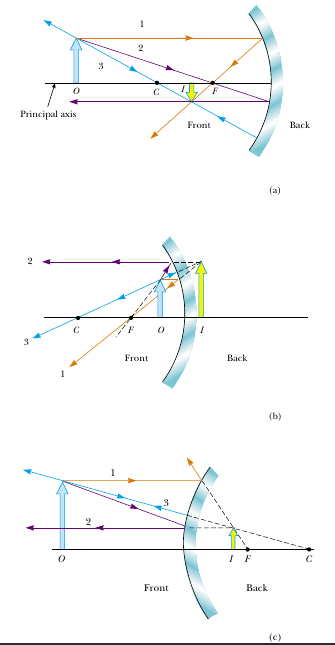
\includegraphics[width=0.5\linewidth]{./3mirrors.png}
  \caption{Cases for object/mirror placement}
  \label{fig:3_mirrors}
  \end{center}
  \par\end{centering}
  \end{figure}

\subsection{Concave Mirrors}
The center of curvature $C$ is located on the principle axis. All paraxial rays (ones that diverge from the principle axis by only a small angle) converge on $I$, so objects placed farther away than $C$ (on the principle axis) produce a \textbf{real} image in front of the mirror. If rays emanating from $O$ instead tend to diverge from the principal axis, spherical aberration is introduced and the image becomes blurred.

Always has a \textbf{positive} focal length -- that is, $F$ is in front of the mirror.
\textbf{3 possible cases:}

\begin{enumerate}
 \item $O > C > F$

 If object is \textit{farther} than $C$, image is \textbf{real, inverted,} and \textbf{reduced} in size.

 \item $C > O > F$

 If the object is \textit{between} $O$ and $F$, its image is \textbf{real, inverted, and enlarged}.

 \item $C > F > O$

 If the object is closer than the focal length, the image is \textbf{virtual, upright,} and \textbf{enlarged}.
\end{enumerate}

\subsection{Convex Mirrors}
Always has \textbf{negative} focal length, where $F$ is located behind the mirror.
Images are always \textbf{virtual, upright,} and \textbf{reduced} in size.
\begin{figure}[h!]
  \begin{centering}
  \begin{center}
  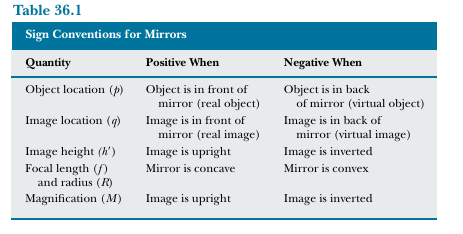
\includegraphics[width=0.5\linewidth]{./mirrorsignconv.png}
  \label{fig:mirror_sign_conventions}
  \caption{Sign Conventions for Mirrors}
  \end{center}
  \par\end{centering}
  \end{figure}

\section{Lenses}

\begin{figure}[h!]
  \begin{centering}
  \begin{center}
  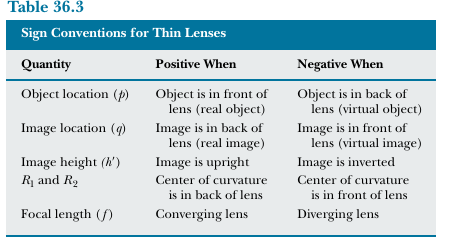
\includegraphics[width=0.5\linewidth]{./lens_conventions.png}
  \caption{Sign conventions for lenses}
  \label{fig:lens_conventions}
  \end{center}
  \par\end{centering}
  \end{figure}

  The Lens-Maker's Equation:
  \begin{align*}
    \frac{1}{f} = (n-1)\left(\frac{1}{R_1} - \frac{1}{R_2}\right)
  \end{align*}

  \begin{figure}[h!]
  \begin{centering}
  \begin{center}
  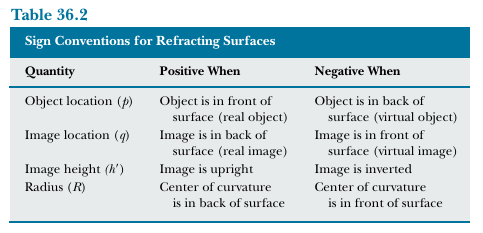
\includegraphics[width=0.5\linewidth]{./refraction_conventions.png}
  \caption{Sign conventions for refracting surfaces.}
  \label{fig:refraction_conventions}
  \end{center}
  \par\end{centering}
  \end{figure}

  \textit{Convention summary:}

  The signs $R$ indicate whether the corresponding surfaces are convex or concave.
  If $R_1$ is positive the first surface is convex, and if $R_1$ is negative the surface is concave.

  The signs are reversed for the back surface of the lens: if $R_2$ is positive the surface is concave, and if $R_2$ is negative the surface is convex.

  \textbf{Comparing Image/Object Rates of Change}

  The thin lens equation can be implicitly differentiated with respect to time to yield this relationship.
  \begin{align*}
   \frac{d}{dt}\left(\frac{1}{p} + \frac{1}{q} = \frac{1}{f}\right) \rightarrow \left(\frac{-1}{p_0^2}\right)p' + \left(\frac{-1}{q_0^2}\right)q' = 0
  \end{align*}



\section{Equations}
\begin{enumerate}
  \item
  Definition of Magnification:
  \begin{align*}
   M = \frac{h'}{h}
  \end{align*}

  \item
  Magnification in a Concave Mirror:
  \begin{align*}
   M = \frac{-q}{p}
  \end{align*}
  $M<1$ indicates that the image is smaller than the object. $-M$ indicates image is inverted.

  \item
  The Mirror Equation:
  \begin{align*}
   \frac{1}{p} + \frac{1}{q} = \frac{1}{f} (\text{ where} f = \frac{R}{2})
  \end{align*}
  Depends only on the curvature of the mirror, and not its material.
  $+q$ denotes an image on the front side of the mirror (real), and vice-versa.
  \end{enumerate}

\section{Homework / Review}
\begin{enumerate}

  \item
    \begin{figure}[h!]
    \begin{centering}
    \begin{center}
    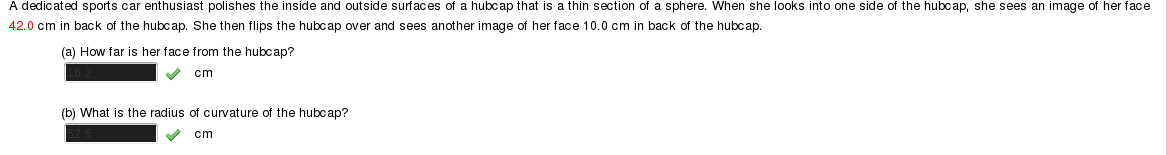
\includegraphics[width=\linewidth]{./hw5.png}
    \label{fig:hw_concave_convex}
    \caption{Convex/Concave Mirrors}
    \end{center}
    \par\end{centering}
    \end{figure}
  Hints: Results in two equations in two unknowns. Near image is convex, far image is concave. $F$ is negative for convex mirrors.

  Solutions: 16.2 cm, 52,5 cm.

  \item
    \begin{figure}[h!]
    \begin{centering}
    \begin{center}
    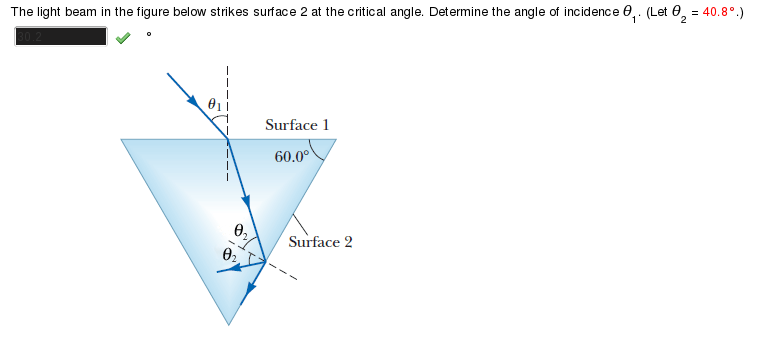
\includegraphics[width=\linewidth]{./prism.png}
    \caption{Determine angle of incidence, given the critical angle inside the prism.}
    \end{center}
    \par\end{centering}
    \end{figure}
  Hints: The sum of interior angles is always $180^{\circ}$. Solve for ratio of indices of refraction. Use Snell's Law.

  Solution: $30.2^{\circ}$.

  \item
    The accommodation limits for a nearsighted person's eyes are 20.0 cm and 81.0 cm. When he wears his glasses, he can see faraway objects clearly. At what minimum distance is he able to see objects clearly?

    \textit{Solution:} Using the lens equation and take $q$ to be the far limit and  $p=\infty$ to find $f$. Then, take $q$ to be the near limit and solve for $p$.
    (26.2 cm)

    \begin{figure}[h!]
    \begin{centering}
    \begin{center}
    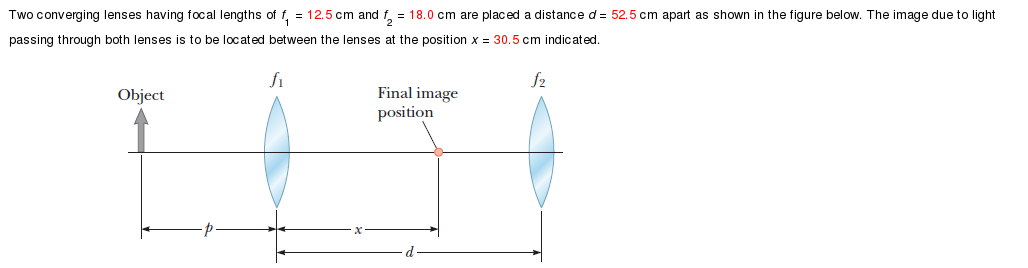
\includegraphics[width=\linewidth]{./hw_double_lenses.png}
    \caption{Two lenses in series}
    \label{fig:hw_double_lenses}
    \end{center}
    \par\end{centering}
    \end{figure}

    \item
      Two converging lenses having focal lengths of $f_1$ = 12.5 cm and $f_2$ = 18.0 cm are placed a distance $d$ = 52.5 cm apart as shown in the figure. The image due to light passing through both lenses is to be located between the lenses at the position $x$ = 30.5 cm indicated.

      At what value of $p$ should an object be placed to produced this image?

      What is the magnification of the final image?

      What is the orientation of the image? Is it real or virtual?

      \hrulefill

      \textit{Solution:}
      Start with the right lens, noting that it must produce a virtual image at $I$. From this, solve for $p_2$ to find the location of the virtual object.

      The distance $q_1$ of the real image produced by the first lens is related to $p_2$, as $q_1 = d - p_2$. This can be used to solve for $p_1$.

      Note sign conventions! $q_2$ is negative, $f$ is positive in both cases since the lenses are converging, and $p$ is positive in both cases.

      $p_1$ = 17.7 cm, $M_T$ = -5.4, the image is enlarged, inverted, and virtual.

      \hrulefill

    \begin{figure}[h!]
  \begin{centering}
  \begin{center}
  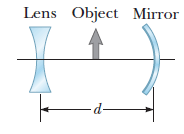
\includegraphics[width=0.25\linewidth]{./hw_lens_mirror.png}
  \caption{Lens/Mirror System}
  \label{fig:lens_mirror}
  \end{center}
  \par\end{centering}
  \end{figure}

    \item
      The object in the figure below is midway between the lens and the mirror, which are separated by a distance $d$ = 24.5 cm.
      The magnitude of the mirror's radius of curvature is 19.5 cm, and the lens has a focal length of -16.8 cm.

      Where is the final image formed by this system?

      Is the image real or virtual? What is its orientation and total magnification?

    \hrulefill

      \textit{Solution: }
      Start with the mirror. Since $p_1$ and $f_1$ are known, solve for $q_1$. Use this as a virtual object for the lens.
      $q_1$ = 47.775 cm, $p_2 = q_1 - d = 23.275$, $q_2 = -60.38$. Note sign conventions: all quantities for mirror are positive, while $f_2$ and $p_2$ are negative.

      So $I$ is 35.9 cm to the right of the mirror, $M_T = 10.1$, and the image is virtual and upright.

    \hrulefill

\end{enumerate}

\end{document}
